\section{Marco Aplicativo}

\subsection{Método de Desarrollo}

Para llevar a cabo el cumplimiento de los objetivos planteados en el Capítulo 2, es necesario definir un
esquema o metodología de trabajo que permita la elaboración de un conjunto de
lineamientos de manera estructurada y organizada. Por lo tanto, se hace uso de el método de
Desarrollo Rápido de Aplicaciones (RAD), el cual permite la iteración rápida y continua
de pequeños objetivos para alcanzar la meta final.

RAD es un proceso de desarrollo de software que
integra un conjunto de técnicas, lineamientos y herramientas que permiten llevar a cabo, en
cortos periodos de tiempo, la implementación de funcionalidades en un sistema, de tal manera que
satisfacen las necesidades del cliente \cite{23}.
Siguiendo esta metodología, el software evoluciona y crece durante el proceso de desarrollo en base a la retro alimentación que se tiene con el cliente.
De esta manera, se realizan múltiples entregas de una tarea que
contiene las nuevas funcionalidades esperadas.
Cada una de estas tareas cuenta con instrumento de documentación al cuál llamaremos historias.
Estas historias describen los detalles técnicos e categorizan las tareas en subgrupos.

Por medio de RAD, fue posible la implementación de la solución al problema previamente planteado, lo cuál fue desarrollada como un servicio web API conformado por:

\begin{itemize}

\item Un modulo de extracción de revisiones de artículos wiki.

\item Un modulo de almacenamiento de datos distribuido por medio de MongoDB.

\item Un modulo de consulta de los artículos wiki extraídos y sus correspondientes revisiones.

\item Y, por último, un modulo de consulta de métricas generales de las revisiones extraídas, incluyendo: totalizaciones, promedios y moda.

\end{itemize}

La siguiente figura representa la vista general de la arquitectura de la aplicación, y como la misma interactuá con
las aplicaciones clientes que consumen el servicio:

\begin{figure}[H]
	\centering
		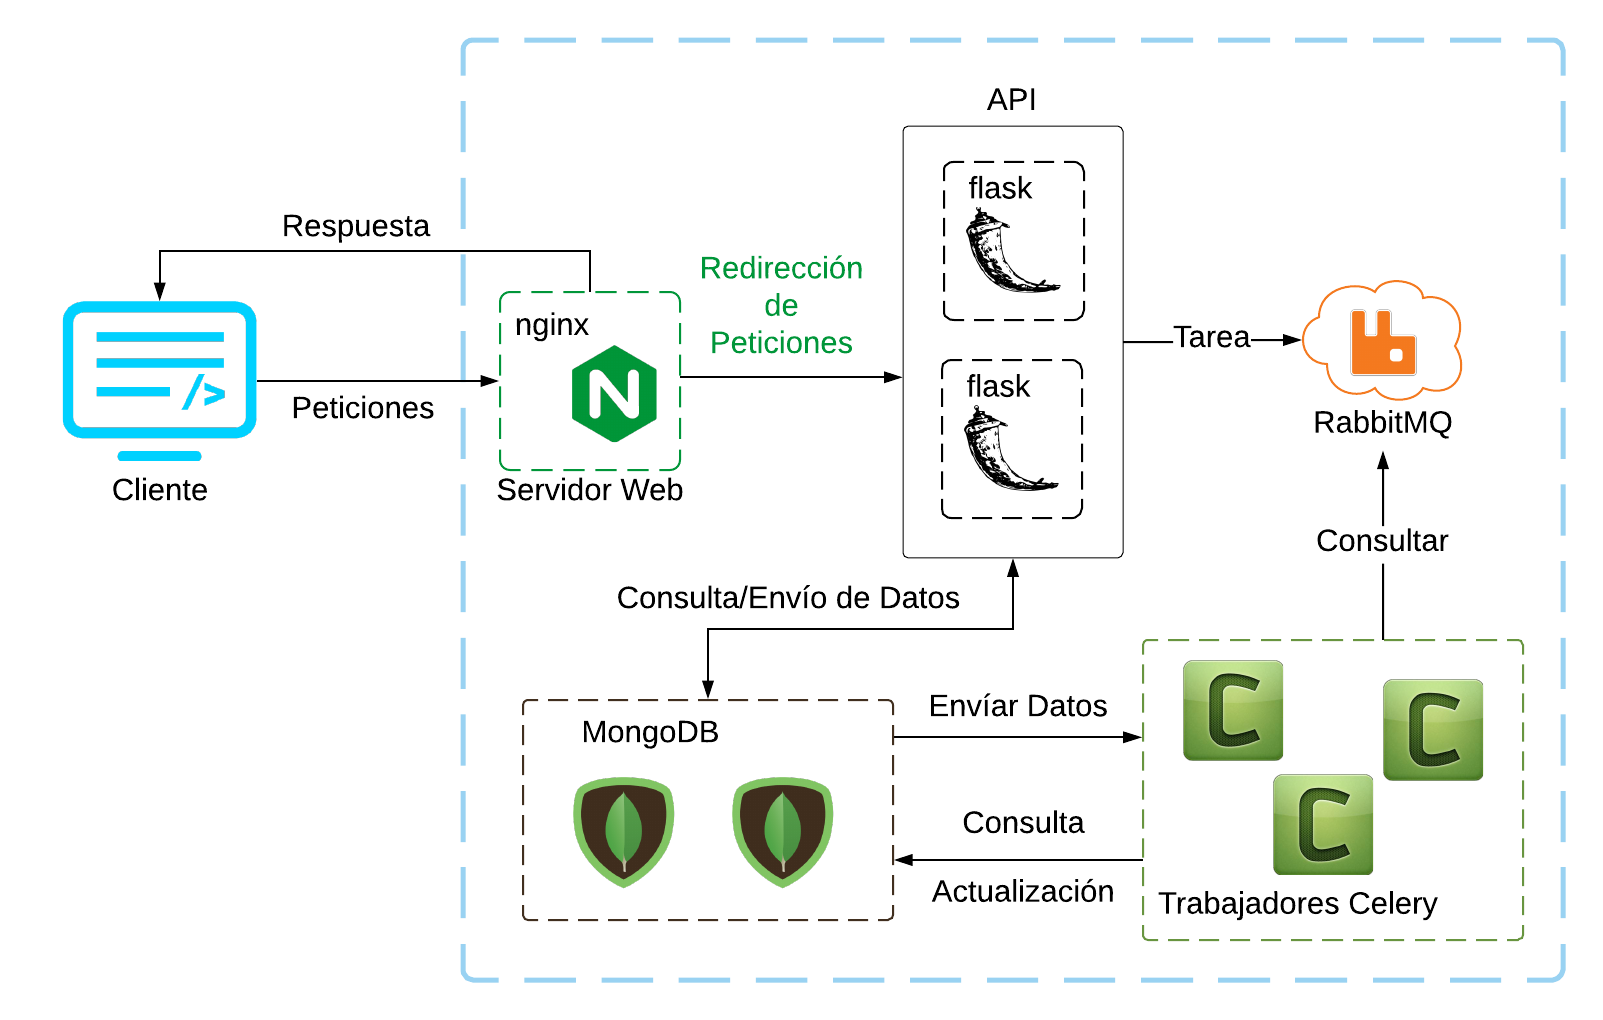
\includegraphics[width=1\textwidth]{figures/diagram_general}
	\caption{Arquitectura general de la aplicación.}
	\label{fig:diagram_general}

\end{figure}

\subsection{Servidor Web}

El servidor web que atiende las solicitudes en primera instancia es Nginx,
el cual funciona como un intermediario entre el cliente y el API que responde dicha solicitud.
Nginx permite balancear la carga de trabajo entre múltiples servidores que contienen la aplicación mediante el algoritmo de round robin,
de tal forma que cada servidor es utilizado de forma equitativa, tal como se muestra en la siguiente figura:

\begin{figure}[H]
	\centering
		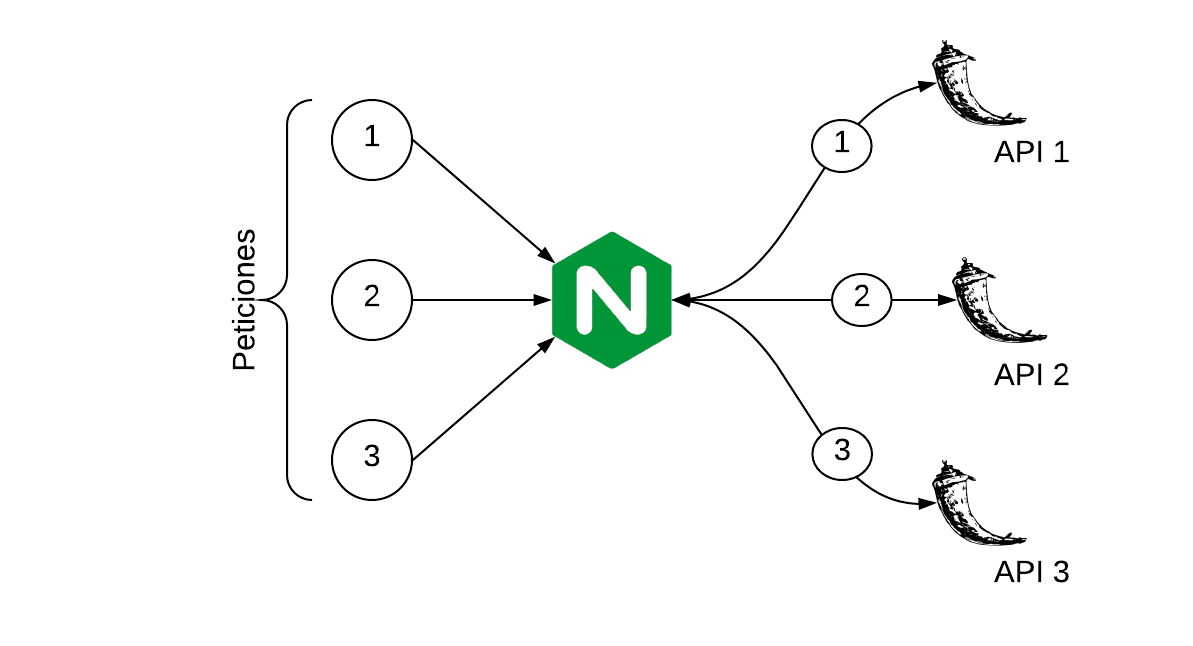
\includegraphics[width=0.9\textwidth]{figures/round_robin}
	\caption{Algoritmo de round robin para la distribución de peticiones de Nginx.}
	\label{fig:round_robin}
\end{figure}

Una vez la petición ha sido reasignada, es atendida por medio del servidor web UWSGI, y en conjunto
con Flask y el resto de las tecnologías incluidas en el API, genera una respuesta de vuelta al cliente.

\subsection{API}

El API diseñado para realizar las labores de extracción y consulta de las revisiones, hace uso del lenguaje de programación Python \texttt{2.7.10} y el uso del framework Flask \texttt{v0.12}.
Ambas tecnologías permiten la asignación de rutas específicas para cada módulo
y la atención de peticiones.

La interacción entre el servicio y una aplicación cliente puede ser apreciada en la figura \ref{fig:diagram_api_1}.

\begin{figure}[H]
	\centering
		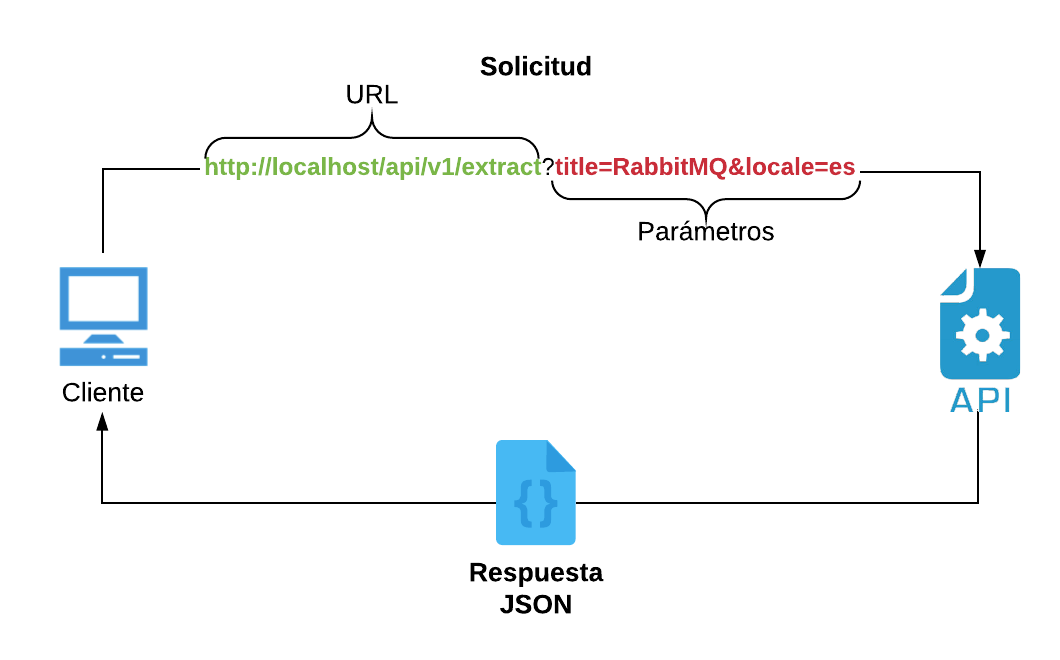
\includegraphics[width=1\textwidth]{figures/diagram_api_1}
	\caption{Interacción entre una aplicación cliente y el API.}
	\label{fig:diagram_api_1}
\end{figure}

Esta interacción se basa en la petición de un recurso o de un proceso, por parte de una aplicación cliente, a una ruta del servidor web (endpoint).
Cada petición puede incluir parámetros opcionales para la paginación, filtración de resultados, como por ejemplo, el idioma del artículo a extraer.

Las rutas de acceso que ofrece el API son las siguientes:

\begin{itemize}
	\item \texttt{/api/v1/articles}. Listado de todos los artículos extraídos.
	\item \texttt{/api/v1/revisions}. Listado de las revisiones de los artículos extraídos.
	\item \texttt{/api/v1/extract}. Extracción de revisiones de artículos wiki.
	\item \texttt{/api/v1/avg}. Cálculo del promedio de revisiones de un artículo por rango fechas.
	\item \texttt{/api/v1/count}. Cálculo de número de revisiones de un artículo por fecha.
	\item \texttt{/api/v1/mode}. Cálculo de las revisiones mas extraídas por rango de fecha.
	\item \texttt{/api/v1/status}. Indica el estado del proceso de extracción.
	\item \texttt{/api/v1/query}. Permite la ejecución de consultas personalizadas a la base de datos.
\end{itemize}

\subsubsection{Extracción de Historiales}

Para la extracción de historiales se hace uso de la ruta de acceso \texttt{/api/v1/extract}, la cual
tiene como parámetros:
\texttt{title}, que se refiere al título del del artículo; \texttt{url}, representa la ruta completa de un artículo, por ejemplo:
\texttt{https://en.wikipedia.org/wiki/The\_Lord\_of\_the\_Rings}; y por último, \texttt{locale}, el cual índica el idioma del artículo y
es completamente opcional, puesto que el sistema asume el inglés como lenguaje por defecto o lo extrae del parámetro
\texttt{url}.
Es necesario proporcionar el parámetro \texttt{url} o \texttt{title} de forma obligatoria para poder llevar a cabo la extracción.

En la siguiente figura se puede apreciar dos ejemplos del uso de los parámetros \texttt{url}, \texttt{title} y \texttt{locale}:

\begin{figure}[H]
	\centering
		
\includegraphics[width=1\textwidth]{figures/extract_url_format}
	\caption{Parámetros para la extracción de historiales.}
	\label{fig:extract_url_format}
\end{figure}

La ejecución de esta tarea se lleva a cabo por medio de Celery y RabbitMQ.
Con estas tecnologías, múltiples computadores ejecutan un proceso de Celery, los
cuales están conectados entre si gracias a RabbitMQ, escuchando constantemente los mensajes entrantes de este servicio.
Una vez recibida la petición por el API, se genera una tarea de extracción por medio de Celery, la cual tiene un identificador único. Esta tarea es encolada en una lista de
espera que es atendida por uno de los trabajadores conectados a RabbitMQ y es ejecutada en segundo plano.
Posteriormente, el API crea una respuesta a la petición generando una ruta para consultar el progreso
del proceso de extracción, la cual luce de la siguiente manera:

\begin{figure}[H]
	\centering
		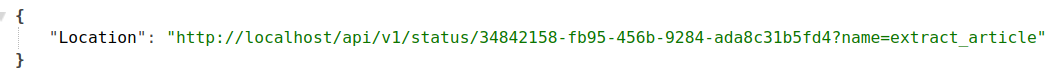
\includegraphics[width=1\textwidth]{figures/extract_response}
	\caption{Respuesta a una petición de extracción de historiales de un artículo.}
	\label{fig:extract_response}
\end{figure}

Durante el proceso de extracción, se realizan peticiones hacia el API de Wikipedia.
Se toma como URL por defecto la dirección https://en.wikipedia.org/w/api.php, en conjunto con diversos parametros, tales como:

\begin{itemize}
	\item \textbf{action}: tipo de petición que se realiza sobre este API, en este caso se hace uso del valor \texttt{query} para indicar que solo se realizará una consulta.

	\item \textbf{format}: formato de la respuesta obtenida, la cual puede ser xml o json.

	\item \textbf{props}: la propiedad del articulo al cual se desea consultar, en este caso se usa el valor \texttt{revisions} para poder extraer el historial de modificaciones del mismo.

	\item \textbf{rvprop}: atributos de la propiedad extraída, los incluidos para esta extracción son los siguientes: ids, flags, timestamp, user, userid, size, sha1, contentmodel, comment, parsedcomment, content, tags.

	\item \textbf{rvlimit}: permite la paginación de los resultados e indica la cantidad de resultados que se quieren obtener por página.

	\item \textbf{newer}: permite ordenar las revisiones de forma ascendete o descendiente acorde a la fecha de creación. Se ordenan de forma descendente usando el valor \texttt{newer}, de esta manera es más rápido extraer las revisiones mas recientes.
\end{itemize}

Justo antes de enviar la solicitud al API de wikipedia, se verifica que el artículo a consultar ya este almacenado en la base de datos, en caso de no estarlo, se almacena indicando la fecha de extracción.
Posteriormente, se extraen sus revisiones, y puesto que la respuesta del API coloca las revisiones mas recientes al principio, el extractor culmina su ejecución una vez determina que alcanzo una revisión que ya ha sido almacenada.
Al almacenar las revisiones en la base de datos, se actualiza el documento del artículo con la fecha de la ultima extracción y el identificador de la revisión extraída, y por ultimo, se actualiza el progreso de la tarea.

En la siguiente figura se puede apreciar un ejemplo de la consulta del progreso de las tareas:

\begin{figure}[H]
	\centering
		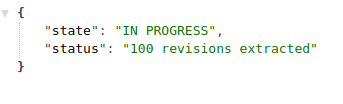
\includegraphics[width=0.8\textwidth]{figures/response_status}
	\caption{Respuesta a una petición para consultar de progreso de una tarea de extracción.}
	\label{fig:response_status}
\end{figure}

La siguiente tabla muestra la historia asociada a la extracción de revisiones:


\renewcommand{\arraystretch}{1.5}
\begin{table}[H]
	\begin{center}
		\begin{tabular}{|l|r|}
			\hline
			\multicolumn{2}{|r|}{\textbf{Historia}} \\
			\hline
			\textbf{Desarrollador} & Marvin Bernal\\
			\hline
			\textbf{Nombre} & Extracción de revisiones por API\\
			\hline
			\textbf{Sección} & Extracción\\
			\hline
			\textbf{Descripción} & \parbox[t]{3in}{Extracción de todas las revisiones de un artículo
				wiki dado su título a través del API que ofrece mediawiki \par
				Se realiza una petición sobre el URL
				\texttt{https://en.wikipedia.org/w/api.php} y se agregan parámetros
				extra, incluyendo el título del artículo, para obtener todos los
				metadatos posibles de una revisión.
				\par
				Cada petición al API obtiene un máximo de 50 revisiones se llevan
				a cabo con una diferencia de 2 segundos.}\\
			\hline
			\textbf{Observaciones} & \parbox[t]{3in}{Se extraen los siguientes datos: id de la revisión, tipo de revisión,
			fecha, nombre de usuario, id de usuario, tamaño, comentarios,
			contenido y etiquetas}\\
			\hline
		\end{tabular}
		\caption{Extracción de Revisiones}
		\label{tab:extract_revisions}
	\end{center}
\end{table}


\subsubsection{Consultas}

El API consta de una ruta de acceso para consultar las revisiones extraídas y
los artículos asociados a través de las rutas \texttt{/api/v1/articles} y \texttt{/api/v1/revisions}.

Para consultar los artículos es posible hacer uso de diversos parámetros de búsqueda,
entre ellas están: los parámetros de paginación \texttt{page} y \texttt{page\_size},
y los parámetros de búsqueda que corresponden a los atributos del artículo,
tales como: \texttt{title}, \texttt{first\_extraction\_date}, \texttt{last\_extraction\_date}, \texttt{last\_revision\_extracted} y \texttt{locale}.

Un ejemplo de la respuesta obtenida por esta ruta puede ser apreciado en la siguiente figura:

\begin{figure}[H]
	\centering
		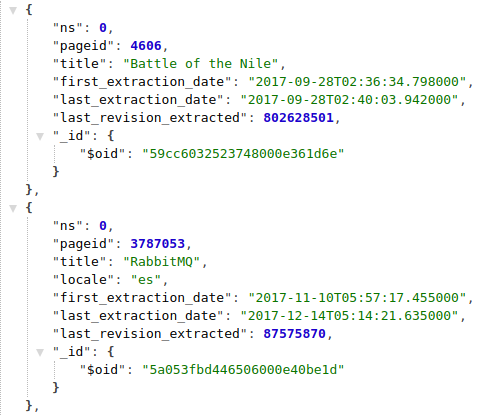
\includegraphics[width=0.8\textwidth]{figures/response_articles}
	\caption{Respuesta a una petición de consulta de artículos.}
	\label{fig:response_articles}
\end{figure}

En el caso de la consulta de las revisiones, adicionalmente a los parámetros de búsqueda, esta el parámetro \texttt{sort} que permite, por fecha de extracción, el
ordenamiento ascendente o descendiente de las revisiones, y la elección de cuales
atributos se desean mostrar por cada revisión.

En la siguiente figura se puede apreciar una respuesta del servidor en la consulta de
revisiones:

\begin{figure}[H]
	\centering
		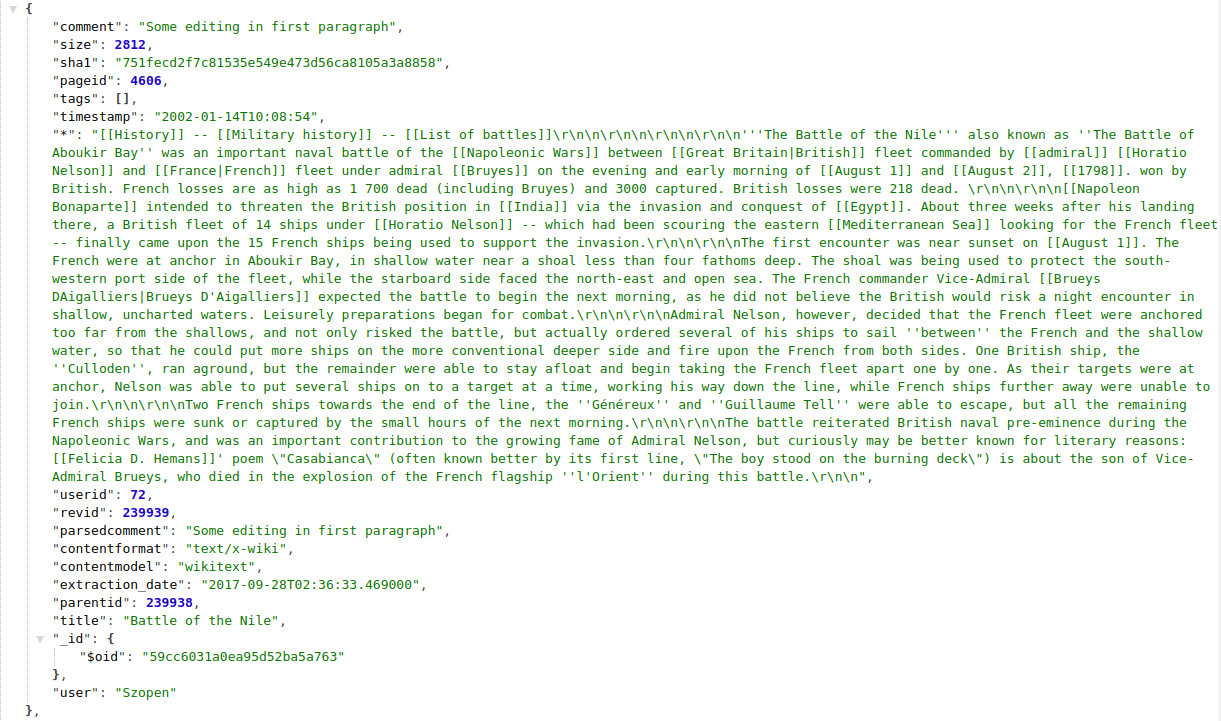
\includegraphics[width=1\textwidth]{figures/response_revisions}
	\caption{Respuesta a una petición de consulta de revisiones.}
	\label{fig:response_revisions}
\end{figure}

Por otro lado, existen mas rutas de acceso al API para la consulta de diversas métricas predefinidas, tales como: promedio, conteo de revisiones y moda.

El cálculo de estas métricas toma como parámetros múltiples atributos
como el título del artículo o la fecha de extracción, para poder filtrar el numero total revisiones de la consulta.
Estos parámetros pasan por un proceso de aceptación, en donde solo son aceptados aquellos que estén ya incluidos en una lista llamada lista blanca, aquellos parámetros que no estén dentro de esta lista son ignorados.
Después de esta etapa, se genera una tarea de Celery para poder ser procesada en segundo plano hasta obtener el resultado.

En las siguientes tablas se puede apreciar con detalle, por medio de sus historias, los filtros aceptados por cada métrica:


\renewcommand{\arraystretch}{1.5}
\begin{table}[H]
	\begin{center}
		\begin{tabular}{|l|r|}
			\hline
			\multicolumn{2}{|r|}{\textbf{Historia}} \\
			\hline
			\textbf{Desarrollador} & Marvin Bernal\\
			\hline
			\textbf{Nombre} & Endpoint para el cálculo de la cantidad de revisiones\\
			\hline
			\textbf{Sección} & Consulta\\
			\hline
			\textbf{Descripción} & \parbox[t]{3in}{Parte del API de la solución distribuida donde el endpoint \texttt{/count}
			recibe como parámetros los atributos para restringir o filtrar el
			rango a tomar en cuenta como resultado. Los argumentos
			disponibles hasta el momento son:\par
				\begin{itemize}

					\item title: título del artículo extraído.
					\item pageid: id del artículo extraído.
					\item user: nombre del usuario que realiza la revisiones.
					\item userid: id del usuario que realiza la revisiones.
					\item tag: una etiqueta determinada que contenga las
					revisiones.
					\item size: el tamaño de la revisión realizada.
					\item sizematch: valor que acompaña a \texttt{size}. Si el valor es
					positivo, se filtrarán todas las revisiones de mayor
					tamaño que el valor de \texttt{size}. Si es negativo, se filtrarán
					todas las revisiones de menor tamaño que el valor de
					\texttt{size}. Si el valor es 0 o no se encuentra en los parámetros
					de la solicitud, se filtrarán todas las revisiones cuyo
					tamaño sea exactamente el valor de \texttt{size}.
					\item date: la fecha exacta en que fueron realizadas las
					revisiones. El formato de fecha utilizado es: \texttt{YYYY-MM-DD}.
					\item datestart: la fecha inicial a partir de la cual fueron
					realizadas las revisiones en un intervalo de tiempo. El
					formato de fecha utilizado es: \texttt{YYYY-MM-DD}. En caso de
					que no exista el parámetro \texttt{dateend} en la solicitud, la fecha final del intervalo será la fecha actual.
					\item dateend: la fecha final hasta la cual fueron realizadas las
					revisiones en un intervalo de tiempo. El formato de
					fecha utilizado es: \texttt{YYYY-MM-DD}. En caso de que no
					exista el parámetro \texttt{datestart} en la solicitud, la fecha
					inicial del intervalo será la fecha de la primera revisión
					del artículo.
				\end{itemize}
				\\
			\hline
			\textbf{Observaciones} & \parbox[t]{3in}{Primero se realiza una comprobación de los parámetros de la
solicitud contra una lista blanca con los parámetros permitidos.
Luego, con los parámetros resultantes, se realiza el
procesamiento a través de una tarea asignada, para luego
devolver el resultado.}\\
			\hline
		\end{tabular}
		\caption{Extracción de Revisiones}
		\label{tab:extract_revisions}
	\end{center}
\end{table}


Por último, el API provee la ruta \texttt{/api/v1/query} que permite ejecutar consultas a la base de datos directamente de los parámetros recibidos por la petición.
El cuerpo de las peticiones realizadas sobre esta ruta debe tener un formato json, en conjunto con el atributo de cabecera
\texttt{content-type} que debe tener como valor \texttt{application/json}.
La estructura del cuerpo de la petición debe coincidir con el formato aceptado para la creación de consultas por medio de PyMongo.
Un ejemplo de este formato puede ser apreciado en la siguiente figura, en donde cada clave de la dupla clave-valor del json representa una función de agregación valida de MongoDB:

\begin{figure}[H]
	\centering
		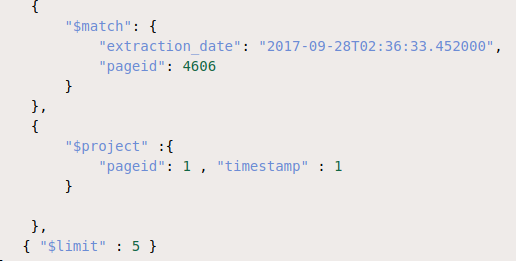
\includegraphics[width=1\textwidth]{figures/query_body_format}
	\caption{Estructura del cuerpo de la petición a la ruta /api/v1/query}
	\label{fig:query_body_format}
\end{figure}

Adicionalmente, la ruta permite especificar la colección de la base de datos a la cual consultar, y de forma opcional,
el formato de fecha de alguna columna en caso de ser necesario.
Un ejemplo, del uso de estos parámetros es el siguiente, en donde se realiza una consulta de la colección llamada revisions:

\begin{figure}[H]
	\centering
		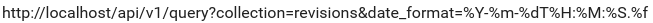
\includegraphics[width=1\textwidth]{figures/query_url}
	\caption{Estructura del cuerpo de la petición a la ruta /api/v1/query}
	\label{fig:query_url}
\end{figure}

Por medio de esta ruta es posible realizar cualquier tipo de consulta sobre la base de datos, y así, obtener métricas
adicionales para su análisis posterior.

\subsection{Revisita}

* Cronjob
* Minipaper, formulas

\subsection{Almacenamiento}

Como fue mencionado en el Capitulo 2, la base de datos utilizada para almacenar las revisiones y artículos wiki, es MongoDB.
A través del proceso de extracción se almacenan dos colleciones:
revisions, que representa las revisiones o historial de modificaciones
del artículo wiki;
 y articles, que se refiere a los artículos de dichas revisiones.



* MongoDB
* Sharding
* Replicas
* Nodos


\subsection{Pruebas}


\subsection{Docker}

* Emulación
* Nodos
* Digital Ocean?
